%Kelompok 3
%Kutub Utara
%
%Andi Syahjaratu Daur - 1154092
%Aditya Pratama Dharma - 1154043
%Bendra Wardhana - 1154015
%Dini Islamiani - 1154039
%Nur Rahmawati - 1154124	
%Pembahasan Dan Isi 

\section{Deskripsi Kutub Utara}	


		Dalam artikel Arctic Monitoring and Assessment Programme (AMAP)  ada beberapa masalah yang ada di dalam 
	kutub utara, yang paling menonjol adalah masalah polusi dan lingkungan.
		
		Kutub Utara sedang mengalami beberapa hal yang paling cepat dan perubahan iklim berat di bumi. Selama 100 tahun, perubahan
	iklim diharapkan untuk mempercepat, memberikan kontribusi untuk fisik utama, ekologi, sosial, dan perubahan ekonomi, banyak yang 
	telah dimulai. Perubahan iklim kutub utara juga akan mempengaruhi seluruh dunia melalui peningkatan pemanasan global dan meningkatnya permukaan laut. 

	Dampak dari Kutub Utara merupakan dataran tinggi penghangat sintesis bahasa dari temuan-temuan kunci Kutub Utara Dampak Perubahan Iklim (ACIA), dirancang 
	untuk dapat diakses untuk para pembuat kebijakan dan publik yang lebih luas. Dalam ACIA adalah secara komprehensif diteliti, benar-benar direferensikan,

	dan evaluasi secara independen dari perubahan iklim kutub utara. Ia telah terlibat sebuah upaya internasional oleh ratusan ilmuwan.
	Dalam artikel Impacts of a Warming Arctic - Arctic Climate Impact Assessment ini menyediakan informasi penting kepada masyarakat dan contemplates-respons 
	untuk salah satu tantangan terbesar pada zaman kita.
	

		Northeast Rusia, dan sungai Mackenzie {130 W. panjang.}, Amerika Barat Laut, dan antara Laut Arctic di utara dan selatan Alaska dan
	Kuriles tengah di selatan. Wilayah ini disajikan sebagai suatu negeri-jembatan antara Eurasia dan Amerika Utara di seluruh Tertiary sehingga kira-kira 5 Ma
	ketika ia diputuskan oleh pembentukan Bering Strait {Marincovich \& Gladenkov 1999, 2001}. Selama Kuartenari, tanah-pembaharuan bridge selama glaciations 
	utama bila tingkat laut jatuh oleh 100-135 m {Hopkins 1973; Clark \& Mencampur 2002}.Northeast Rusia dan Amerika Barat Laut {Alaska dan Yukon} tetap bebas es 
	selama Kuartenari glaciations dan melayani sebagai refugium utara besar-besaran untuk kutub utara dan boreal biota. Wilayah ini Beringia Hultén dipanggil dan
	didefinisikan sebagai kawasan antara Sungai Lena {125 E. panjang.}, Northeast Rusia, dan sungai Mackenzie{130 W. panjang.}, 
	Amerika Barat Laut, dan antara Laut Arctic di utara dan selatan Alaska dan Kuriles tengah di selatan. Wilayah ini disajikan sebagai suatu negeri-jembatan antara 
	Eurasia dan Amerika Utara di seluruh Tertiary sehingga kira-kira 5 Ma ketika ia diputuskan oleh pembentukan Bering Strait {Marincovich \& Gladenkov 1999, 2001}. 
	Selama Kuartenari, tanah-pembaharuan bridge selama glaciations utama bila tingkat laut jatuh oleh 100-135 m {Hopkins 1973; Clark \& Mencampur 2002}.
	
\subsection{Kutub Utara Tahun ini}

		Dalam Kuartenari {kira-kira 2 Ma hingga sekarang} distribusi dan komposisi kutub utara flora ini sangat dipengaruhi oleh terlebih dahulu dan mundur dari 
	lapisan-lapisan es. Secara tradisional, ia berpikir bahwa selama periode seret nya proses semua wilayah utara tertutup oleh es ke sejauh serupa dan bahwa
	binatang dan tumbuhan kutub utara bermigrasi ke selatan memajukan lembaran-es untuk bertahan hidup di selatan refugia {Darwin tahun 1859; Hooker tahun 1862}.

	Namun, keyakinan ini menghadapi tantangan dalam 1937 oleh bahasa Swedia botanis, Eric Hultén, dalam bukunya garis besar tentang sejarah Kutub Utara dan 
	Boreal Biota selama periode divisi kuartenari. Hultén menarik pada bukti geologi dan tubuh yang luas dari bukti phytogeographical sendiri, untuk mengusulkan
	bahwa kebanyakan dari Northeast Rusia dan Amerika Barat Laut (Alaska dan Yukon) tetap bebas es selama Kuartenari glaciations dan melayani sebagai refugium 
	utara besar-besaran untuk kutub utara dan boreal biota {Gbr. 1}. Wilayah ini Beringia Hultén dipanggil dan didefinisikan sebagai kawasan antara Sungai Lena 
	{125 E. panjang.}
		Kutub Utara tahun ini terdiri dari kira-kira 1.500 spesies flora dan yang relatif baru asal usul {Murray 1995}. Perguruan Tinggi di sebagian besar {65-2 Ma}, 
	hutan tumbuh di ketika latitude tinggi di Kutub Utara {Murray 1995; McIver \& Basinger 1999} dan tundra tidak muncul hingga akhir Pliocene {Salasila Matius \& Ovenden 1990}.
	Pada awalnya tundra ini disebarluaskan discontinuously, tetapi sebuah sabuk circumarctic hadir dengan 3 Ma {Salasila Matius 1979}. 

	Sedikit yang mengetahui tentang asal-usul tumbuhan kutub utara, walaupun seandainya banyak tanaman tersebut berasal dari saham nenek moyang yang terjadi di gunung-gunung yang tinggi, di sebelah selatan di Asia dan Amerika Utara {Hultén 1937; Tolmachev 1960; Weber 1965; Hedberg 1992; Murray 1995}. Gunung ini membentuk 
	bagian dari berkisar antara terhubung ke Kutub Utara, di sepanjang tanaman yang dapat bermigrasi ke arah utara, seperti suhu global yang turun secara signifikan dari 

	pertengahan Miocene dan seterusnya {Lear et al. 2000; Zachos et al. 2001}. Selain itu, beberapa tanaman kutub utara mungkin berasal dari shrubby dan elemen-elemen 
	herbaceous hutan kutub utara yang menduduki Tersier membuka, dan riparian {40-2}-habis sama sekali habitat dataran tinggi di Kutub Utara selama akhir.
	
\begin{figure}[ht]

\centerline{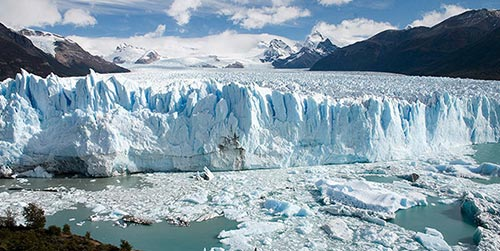
\includegraphics[width=.5\textwidth]{figures/arctic.jpg}}
\caption{Gambar Arctic atau kutub utara.}	

\label{Kutub_Utara}
\end{figure}
	
\subsection{Pemanasan di kutub utara}

		Metana di dalam Atmosfer kutub utara telah meningkat dengan tajam sebanyak 33% dalam kurun 5 tahun tanah es yang mencair di siberia telah melepaskan 5x 
	jumlah metana dari yang sebelum nya di prediksi permafrost dangkal bawah laut pada kutub utara juga menunjukkan ketidakstabilan dan melepaskan jumlah metana
	yang banyak padang rumput pada kutub utara pada saat ini sudah mengeluarkan lebih banyak metana dan nitrogen oksida dari perkiraan yang sebelumnya ilmuwan 
	telah memberi nama pencairan kutub utara dengan nama bom waktu yang berdetak, Kutub utara memanas dua kali lebih cepat di bandingkan tempat lain yang berada
	di bumi tanpa es yang melindungi untuk memantulkan sinar matahari , di dunia terdapat dua lapisan es besar yaitu Greenland dan kutub selatan Kutub utara merupakan
	negara yang mustahil untuk di tempati makhluk hidup namun juga terdapat beberapa spesies fauna yang dapat hidup di sana salah satu nya adalah beruang kutub
	meski memiliki tubuh yang besar beruang kutub mampu berenang selama berhari-hari di perairan terbuka dan sanggup menjangkau jarak ratusan kilometer .

\begin{figure}[ht]
\centerline{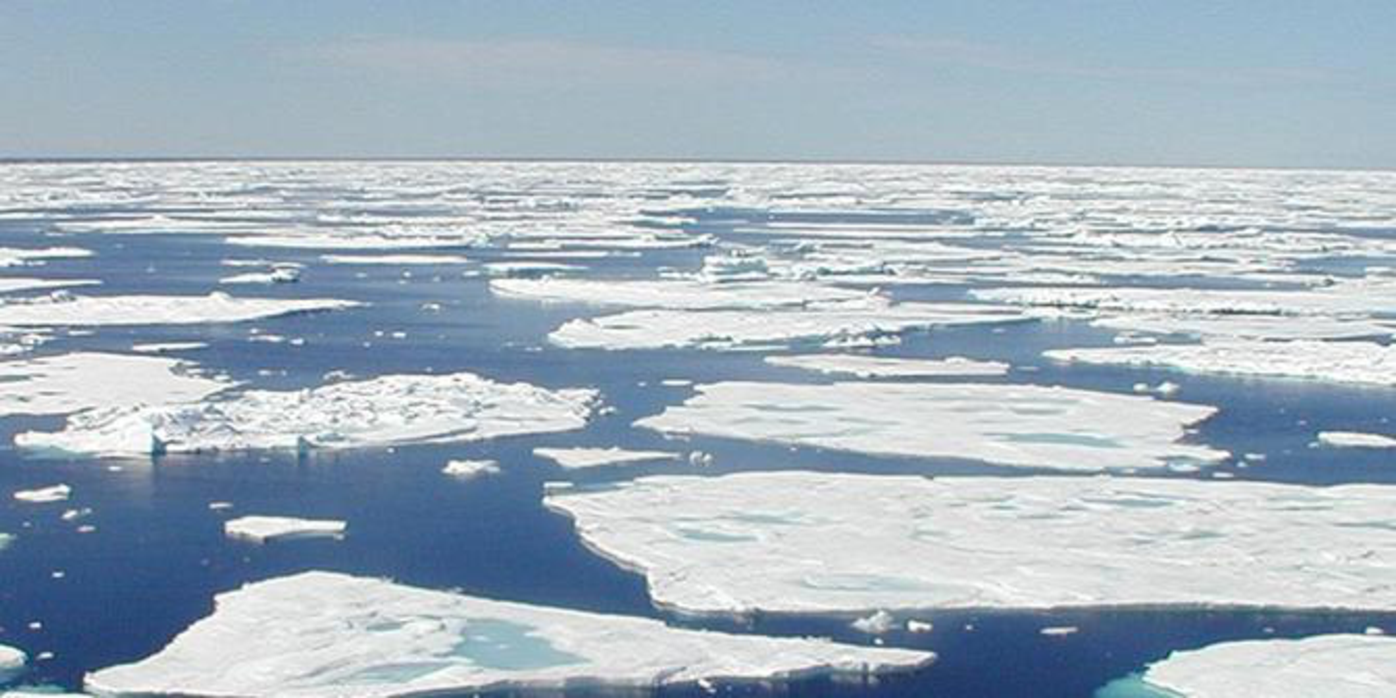
\includegraphics[width=0.5\textwidth]{figures/arctic1.pdf}}
\caption{Menjelaskan tentang pemanasan kutub utara.}	

\label{Pemanasan_Kutub_Utara}
\end{figure}




\subsection{Kutub Utara}	
Dari 2 meter lebih pada 50 tahun 
	mendatang. Upaya untuk mengatasi tantangan perubahan iklimdan kenaikan permukaan laut tersebut, kota Rotterdam telah membangun beberapa struktur terapung 
	berdesain unik dan menarik, Dan Menurut nanang rianto dampak pencairan es di Kutub Utara dan Selatan akibat pemanasan global dan gejala penurunan elevasi
	tanah (land subsidence).
	
		Kutub utara diramalkan akan punah karena habitatnya yang mengecil. Bobot hewan disana mengalami penyusutan yang signifikan dalam beberapa decade terakhir ini. Makanan beruang adalah ikan,Mereka mencarinya dengan membuat lubang di lapisan es sehingga ketika ada ikan lewat langsung disambarnya.sekarang 

	jangankan membuat lubang mencari tempat berpijak saja susah karena banyaknya es yang mencair sehingga beruang harus sering melompat berpindah balok es.
	Tak jarang pun ikan susah ditangkap. Beruang kutub harus berenang bermil-mil demi mendapatkan tempat baru, dan ini berisiko besar karena domain beruang
	kutub bukanlah di laut.
	
	

\subsubsection {Kutub Utara}
		Kutub utara magnet bumi untuk di interpretasi. Hasil interpretasi kualitatif menunjukkan bahwa pada peta anomali regional terdapat anomali dipole magnetik

	yang membentang dari arah barat daya ke timur laut Semenanjung Muria, Peta anomali lokal menunjukkan dua buah anomali dipole magnetik yang membentang dari 
	arah barat laut ke tenggara di sebelah utara dan barat kompleks Gunung api Muria, dan satu pasang dipole magnetik di tenggara Gunung api Muria Hasil 
	interpretasi kuantitatif yang dilakukan dengan menggunakan software Mag2DC for Windows. Pada anomali regional dan anomali lokal yang direduksi ke kutub 
	terdapat sebuah sesar di sebelah tenggara gunungapi Muria, tepatnya pada daerah Maar Gunung Rowo. Struktur geologi bawah permukaan daerah Gunung api Muria 
	dan Maar Gunung Rowo berdasarkan harga suseptibilitas batuan dikontrol oleh batuan vulkanik yang terdiri dari andesit dari satuan batuan Lava Muria, tufa 
	dari satuan batuan Tuf Muria, batu pasir tufaan dari formasi Patiayam, batugamping dari formasi Bulu, dan batulempung dari formasi Ngrayong. Pada kedalaman
	7-15 km di bawah permukaan terdapat batuan vulkanik dan vulkanik klastik yang merupakan batuan dasar penyusun Semenanjung Muria.
	
\subsubsection{kutub utara magnet di interpretasi}
		Kutub utara magnet bumi untuk di interpretasi. Hasil interpretasi kualitatif menunjukkan bahwa pada peta anomali regional terdapat anomali dipole 
	magnetik yang membentang dari arah barat daya ke timur laut Semenanjung Muria, Peta anomali lokal menunjukkan dua buah anomali dipole magnetik yang 
	membentang dari arah barat laut ke tenggara di sebelah utara dan barat kompleks Gunung api Muria, dan satu pasang dipole magnetik di tenggara Gunung api
	Muria Hasil interpretasi kuantitatif yang dilakukan dengan menggunakan software Mag2DC for Windows. Pada anomali regional dan anomali lokal yang direduksi
	ke kutub terdapat sebuah sesar di sebelah tenggara gunungapi Muria, tepatnya pada daerah Maar Gunung Rowo. Struktur geologi bawah permukaan daerah 
	Gunung api Muria dan Maar Gunung Rowo berdasarkan harga suseptibilitas batuan dikontrol oleh batuan vulkanik yang terdiri dari andesit dari 
	satuan batuan Lava Muria, tufa dari satuan batuan Tuf Muria, batu pasir tufaan dari formasi Pati ayam, batu gamping dari formasi Bulu, dan 
	batu lempung dari formasi Ngrayong. Pada kedalaman 7-15 km di bawah permukaan terdapat batuan vulkanik dan vulkanik klastik yang merupakan 
	batuan dasar penyusun Semenanjung Muria.
	
\subsubsection {kutub utara terendam}

		Menurut artikel Fatmasari Savitri, Eddy Prianto, Erni Setyowati kutub utara dan selatan bumi akan terendam lebih dari 2 meter lebih pada 50 
	tahun mendatang. Upaya untuk mengatasi tantangan perubahan iklim dan kenaikan permukaan laut tersebut, kota Rotterdam telah membangun beberapa 
	struktur terapung berdesain unik dan menarik. 

\subsubsection {kepunahan habitat kutub utara}
		Kutub utara diramalkan akan punah karena habitatnya yang mengecil. Bobot hewan itu mengalami penyusutan signifikan dalam dekade akhir ini.
	Makanan beruang adalah ikan, Mereka mencarinya dengan membuat lubang di lapisan es sehingga ketika ada ikan lewat langsung di sambarnya. Sekarang jangankan membuat lubang mencari tempat berpijak saja susah karena banyaknya es yang mencair sehingga beruang harus sering melompat berpindah balok es. Tak jarang pun ikan susah ditangkap.beruang kutub harus berenang bermil-mil demi mendapatkan tempat baru, dan ini berisiko besar karena domain beruang kutub bukanlah dilaut.
	
		


